% FYP Presentation — All-Weather Smart Vehicle Gate System
% Compile: pdflatex fyp_presentation.tex (run twice for TOC)
\documentclass[aspectratio=169,11pt]{beamer}

\usetheme{Madrid}
\usecolortheme{default}
\setbeamertemplate{navigation symbols}{}
\setbeamertemplate{footline}[frame number]

\usepackage[T1]{fontenc}
\usepackage[utf8]{inputenc}
\usepackage{lmodern}
\usepackage{graphicx}
\usepackage{booktabs}
\usepackage{tabularx}
\usepackage{amsmath}
\usepackage{tikz}
\usetikzlibrary{arrows.meta,positioning,fit,shapes.geometric,calc}
\usepackage{listings}
\usepackage{xcolor}
\usepackage{multicol}
\usepackage{hyperref}

\hypersetup{colorlinks=true, linkcolor=blue!70!black, urlcolor=blue!70!black}

% Colors matching project diagrams
\definecolor{navycolor}{RGB}{30,58,95}
\definecolor{accentorange}{RGB}{255,102,0}
\definecolor{boxinput}{RGB}{245,245,245}
\definecolor{boxprep}{RGB}{200,230,255}
\definecolor{boxdetect}{RGB}{255,220,180}
\definecolor{boxchar}{RGB}{255,200,200}
\definecolor{boxvmmr}{RGB}{220,200,255}
\definecolor{boxpost}{RGB}{200,255,200}
\definecolor{boxdeploy}{RGB}{180,230,230}
\definecolor{boxserver}{RGB}{230,220,250}
\definecolor{grantgreen}{RGB}{40,160,80}
\definecolor{denyred}{RGB}{200,50,50}
\definecolor{alertorange}{RGB}{230,130,30}

\setbeamercolor{structure}{fg=navycolor}
\setbeamercolor{frametitle}{bg=navycolor, fg=white}
\setbeamercolor{title}{fg=navycolor}
\setbeamercolor{block title}{bg=navycolor, fg=white}
\setbeamercolor{block body}{bg=blue!5}

\lstset{
  basicstyle=\ttfamily\scriptsize,
  breaklines=true,
  frame=single,
  backgroundcolor=\color{gray!8},
  keywordstyle=\color{blue!70!black},
  stringstyle=\color{green!40!black},
}

\title[Smart Vehicle Gate FYP]{Automatic Vehicle Gate Access System\\in All-Weather Conditions}
\subtitle{License Plate Recognition + Vehicle Make \& Model Recognition}
\author{Ali Raza Chaudhry \and Abdul Hadi}
\institute{COMSATS University Islamabad, Lahore Campus\\B.S. Computer Engineering\\Supervisor: Dr.\ Taimoor Naeem}
\date{Final Year Project Defense --- 2025}

\begin{document}

%==============================================================================
\begin{frame}
  \titlepage
\end{frame}

%==============================================================================
\begin{frame}{Outline}
  \tableofcontents
\end{frame}

%==============================================================================
\section{Introduction}
%==============================================================================

\begin{frame}{Problem Statement}
  \begin{block}{Challenge}
    Outdoor vehicle gates must identify \textbf{license plates} and verify \textbf{vehicle identity}
    under fog, rain, glare, and night --- yet many systems rely on \textbf{plate-only} decisions
    vulnerable to misreads and cloned plates.
  \end{block}
  \vspace{0.4em}
  \begin{columns}[T]
    \column{0.48\textwidth}
    \textbf{Limitations of existing systems:}
    \begin{itemize}
      \item Poor performance in adverse weather
      \item Plate-only authorization (spoofing risk)
      \item Cloud-dependent (latency, privacy)
      \item Fragmented LPR + VMMR pipelines
    \end{itemize}
    \column{0.48\textwidth}
    \textbf{Our solution:}
    \begin{itemize}
      \item Weather-aware preprocessing
      \item Dual YOLOv8n LPR pipeline
      \item EfficientNet-B4 VMMR (245 classes)
      \item Dual-modality gate policy
      \item Edge AI on Orange Pi 5 Pro
    \end{itemize}
  \end{columns}
\end{frame}

\begin{frame}{Objectives \& Contributions}
  \begin{enumerate}
    \item Train \textbf{YOLOv8n} for license plate detection (LPD)
    \item Train \textbf{YOLOv8n} for character/digit detection (38 classes)
    \item Train \textbf{EfficientNet-B4} for 245 make--model families (VMMR)
    \item Integrate fog, rain, and night preprocessing before inference
    \item Implement dual-modality access control (plate + make/model)
    \item Deploy on \textbf{Orange Pi} with web dashboard for monitoring
  \end{enumerate}
  \vspace{0.5em}
  \begin{alertblock}{Novelty}
    Coupled pipeline: weather restoration $\rightarrow$ dual YOLO LPR $\rightarrow$ VMMR
    $\rightarrow$ JSON $\rightarrow$ allow/deny/alert policy --- reproducible end-to-end.
  \end{alertblock}
\end{frame}

%==============================================================================
\section{System Architecture}
%==============================================================================

\begin{frame}{High-Level System Architecture}
  \centering
  \resizebox{0.95\textwidth}{!}{%
  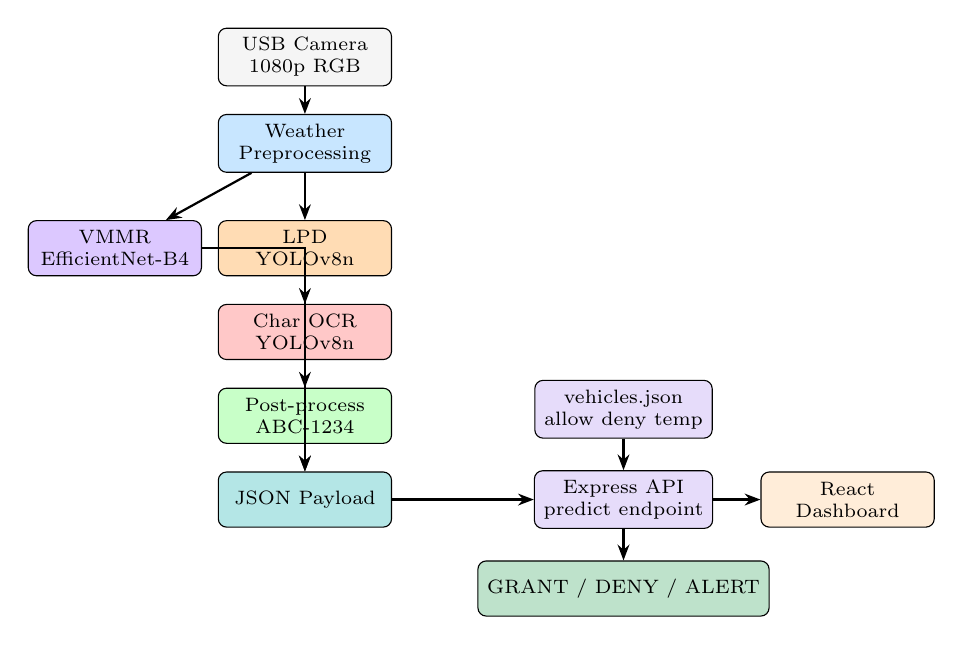
\begin{tikzpicture}[
    node distance=0.35cm and 0.5cm,
    box/.style={draw, rounded corners=3pt, align=center, font=\scriptsize,
                minimum width=2.2cm, minimum height=0.7cm},
    arr/.style={-{Stealth[length=2mm]}, thick}
  ]
    \node[box, fill=boxinput] (cam) {USB Camera\\1080p RGB};
    \node[box, fill=boxprep, below=of cam] (pre) {Weather\\Preprocessing};
    \node[box, fill=boxvmmr, below left=0.6cm and 0.2cm of pre] (vmmr) {VMMR\\EfficientNet-B4};
    \node[box, fill=boxdetect, below=0.6cm of pre] (lpd) {LPD\\YOLOv8n};
    \node[box, fill=boxchar, below=of lpd] (ocr) {Char OCR\\YOLOv8n};
    \node[box, fill=boxpost, below=of ocr] (post) {Post-process\\ABC-1234};
    \node[box, fill=boxdeploy, below=of post] (json) {JSON Payload};
    \node[box, fill=boxserver, right=1.8cm of json] (api) {Express API\\predict endpoint};
    \node[box, fill=boxserver, above=0.4cm of api] (db) {vehicles.json\\allow deny temp};
    \node[box, fill=grantgreen!30, below=0.4cm of api] (gate) {GRANT / DENY / ALERT};
    \node[box, fill=boxdetect!50, right=0.6cm of api] (dash) {React\\Dashboard};

    \draw[arr] (cam) -- (pre);
    \draw[arr] (pre) -- (vmmr);
    \draw[arr] (pre) -- (lpd);
    \draw[arr] (lpd) -- (ocr);
    \draw[arr] (ocr) -- (post);
    \draw[arr] (vmmr.east) -| ($(json.north)+(0,0.3)$) -- (json);
    \draw[arr] (post) -- (json);
    \draw[arr] (json) -- (api);
    \draw[arr] (db) -- (api);
    \draw[arr] (api) -- (gate);
    \draw[arr] (api) -- (dash);
  \end{tikzpicture}%
  }
\end{frame}

\begin{frame}{End-to-End Data Flow}
  \small
  \begin{enumerate}
    \item \textbf{Capture:} USB camera acquires full vehicle frame (RGB)
    \item \textbf{Preprocess:} Apply fog / rain / night restoration (or pass-through)
    \item \textbf{Stage 0 --- VMMR:} Classify make--model on full preprocessed image
    \item \textbf{Stage 1 --- LPD:} Detect plate bounding box ($\text{conf} \geq 0.25$)
    \item \textbf{Stage 2 --- OCR:} Detect characters on cropped plate (+4\,px padding)
    \item \textbf{Post-process:} Sort left$\rightarrow$right, format as \texttt{LETTERS-DIGITS}
    \item \textbf{Deploy:} Orange Pi builds JSON, HTTP POST to web server
    \item \textbf{Policy:} Match plate + make/model against database $\rightarrow$ gate action
  \end{enumerate}
  \vspace{0.3em}
  \begin{exampleblock}{Edge performance (Orange Pi 5 Pro CPU)}
    Total latency: \textbf{700--1000\,ms/image} ($\sim$1\,FPS) --- acceptable for single-lane gate access.
  \end{exampleblock}
\end{frame}

%==============================================================================
\section{Input \& Preprocessing}
%==============================================================================

\begin{frame}{Input Image Handling}
  \begin{columns}[T]
    \column{0.55\textwidth}
    \textbf{Sources:}
    \begin{itemize}
      \item USB 1080p camera at gate lane (live)
      \item Batch image upload (JPG, PNG, BMP, WEBP, TIF)
    \end{itemize}
    \textbf{Processing:}
    \begin{itemize}
      \item Convert to RGB: \texttt{PIL.Image.convert('RGB')}
      \item Unsupported formats re-saved as JPEG
      \item Original resolution preserved; models resize internally
    \end{itemize}
    \textbf{Hardware:}
    \begin{itemize}
      \item Orange Pi 5 Pro (16\,GB RAM)
      \item 5V 5A USB-C power supply
      \item Optional GPIO relay for physical gate
    \end{itemize}
    \column{0.42\textwidth}
    \begin{block}{Preprocessing Modes}
      \begin{tabular}{@{}ll@{}}
        \toprule
        \textbf{Flag} & \textbf{Filter} \\
        \midrule
        \texttt{none} & Pass-through \\
        \texttt{auto} & Auto-detect weather \\
        \texttt{fog} & DCP defog \\
        \texttt{rain} & Vertical median \\
        \texttt{night} & CLAHE + gamma \\
        \bottomrule
      \end{tabular}
    \end{block}
  \end{columns}
\end{frame}

\begin{frame}{Fog / Haze Removal --- Dark Channel Prior}
  \textbf{Function:} \texttt{defog\_image()} --- runs \emph{before} all AI models
  \begin{columns}[T]
    \column{0.58\textwidth}
    \small
    \begin{enumerate}
      \item Compute dark channel (13$\times$13 morphological erosion)
      \item Estimate atmospheric light (top 0.1\% darkest pixels)
      \item Transmission map + guided filter ($r{=}50$, $\varepsilon{=}10^{-3}$)
      \item Scene radiance recovery: $(I - A) / t + A$
      \item Residual haze removal on bright low-variance regions
      \item Gray-world color balance
      \item Adaptive gamma correction ($\gamma \in [0.6, 1.8]$)
      \item CLAHE on LAB L-channel (clip=2.5, 8$\times$8 tiles)
      \item HSV saturation boost ($\times 1.2$)
      \item Bilateral filter + unsharp mask
    \end{enumerate}
    \column{0.40\textwidth}
    \begin{block}{Why classical CV?}
      \begin{itemize}
        \item No extra DL model to train
        \item Fast on Orange Pi CPU
        \item Interpretable parameters
        \item Works without paired training data
      \end{itemize}
    \end{block}
    \begin{alertblock}{Key idea}
      Dark pixels in outdoor haze reveal depth; dehazing restores plate edges and vehicle texture.
    \end{alertblock}
  \end{columns}
\end{frame}

\begin{frame}{Rain \& Night Preprocessing}
  \begin{columns}[T]
    \column{0.48\textwidth}
    \textbf{Rain Removal --- \texttt{derain\_image()}}
    \begin{itemize}
      \item Edge-protection mask (bilateral + Canny)
      \item Vertical median filters: 15, 11, 7 px kernels
      \item Brightening guard (prevents halos on glyphs)
      \item Rain spot detection (area 2--250\,px)
      \item Telea inpainting ($r{=}3$)
    \end{itemize}
    \column{0.48\textwidth}
    \textbf{Night Enhancement --- \texttt{preprocess\_night()}}
    \begin{itemize}
      \item Black-level lift on LAB L-channel (up to +55)
      \item Adaptive CLAHE (clip 4.5--8.5, 6$\times$6)
      \item Adaptive gamma ($\gamma \in [0.28, 0.62]$)
      \item Global gain if mean $< 100$ ($\times 1.0$--$2.5$)
      \item HSV saturation $\times 1.55$
      \item Unsharp mask for edge recovery
    \end{itemize}
  \end{columns}
  \vspace{0.5em}
  \centering
  \textit{All three branches feed the same downstream YOLO + EfficientNet weights.}
\end{frame}

%==============================================================================
\section{AI Models}
%==============================================================================

\begin{frame}{Model Summary}
  \centering
  \scriptsize
  \begin{tabular}{@{}lcccccc@{}}
    \toprule
    \textbf{Stage} & \textbf{Model} & \textbf{Classes} & \textbf{Input} & \textbf{Epochs} & \textbf{Weight file} & \textbf{mAP / Acc.} \\
    \midrule
    LPD & YOLOv8n & 1 (plate) & 384 & 50 & \texttt{plate\_best.pt} & mAP@0.5 = 98.1\% \\
    Char OCR & YOLOv8n & 38 & 640 & 100 & \texttt{char\_best.pt} & mAP@0.5 = 98.1\% \\
    VMMR & EfficientNet-B4 & 245 & 380 & 50 & \texttt{efficientnet\_b4\_best.pth} & Top-1 = 96.2\% \\
    \bottomrule
  \end{tabular}
  \vspace{0.8em}

  \begin{columns}[T]
    \column{0.32\textwidth}
    \begin{block}{LPD Dataset}
      Roboflow \emph{License Plate Project} v1
    \end{block}
    \column{0.32\textwidth}
    \begin{block}{OCR Dataset}
      Roboflow \emph{My First Project} v4 (Pakistani plates)
    \end{block}
    \column{0.32\textwidth}
    \begin{block}{VMMR Dataset}
      Custom 245-class folder dataset (17{,}254 test images)
    \end{block}
  \end{columns}
\end{frame}

\begin{frame}[fragile]{Stage 1 --- License Plate Detection (YOLOv8n)}
  \begin{columns}[T]
    \column{0.52\textwidth}
    \textbf{Architecture:} YOLOv8 nano (Ultralytics)
    \begin{itemize}
      \item Single detection class: \texttt{plate}
      \item Pretrained on COCO, fine-tuned on Roboflow v1
      \item Training: 50 epochs, batch=32, imgsz=384
      \item Inference: $\text{conf} \geq 0.25$, NMS IoU=0.7
    \end{itemize}
    \textbf{Output:} Bounding box $(x_1, y_1, x_2, y_2)$
    \begin{lstlisting}
plate_results = plate_model.predict(
    source=img_np, conf=0.25)
    \end{lstlisting}
    \column{0.45\textwidth}
    \begin{block}{Metrics (Epoch 50)}
      \begin{tabular}{@{}lr@{}}
        Precision & \textbf{98.50\%} \\
        Recall    & \textbf{95.53\%} \\
        mAP@0.5   & \textbf{98.07\%} \\
        mAP@0.5:0.95 & 70.73\% \\
      \end{tabular}
    \end{block}
    \begin{exampleblock}{Why YOLOv8n?}
      Small ($\sim$6\,MB), fast on Pi CPU (80--200\,ms), sufficient accuracy for gate LPD.
    \end{exampleblock}
  \end{columns}
\end{frame}

\begin{frame}{Stage 2 --- Character / Digit Detection (YOLOv8n)}
  \begin{columns}[T]
    \column{0.52\textwidth}
    \textbf{Task:} Detect individual characters on cropped plate
    \begin{itemize}
      \item 38 classes: digits 0--9, letters A--Z, \texttt{YY}, \texttt{a}
      \item Training: 100 epochs, batch=16, imgsz=640
      \item Each character = one detection box (not seq2seq OCR)
    \end{itemize}
    \textbf{Advantages over traditional OCR:}
    \begin{itemize}
      \item Handles skewed / dirty plates
      \item No separate OCR engine dependency
      \item End-to-end trainable with plate data
    \end{itemize}
    \column{0.45\textwidth}
    \begin{block}{Metrics (Epoch 100)}
      \begin{tabular}{@{}lr@{}}
        Precision & \textbf{98.99\%} \\
        Recall    & \textbf{96.88\%} \\
        mAP@0.5   & \textbf{98.07\%} \\
        mAP@0.5:0.95 & 76.11\% \\
      \end{tabular}
    \end{block}
    \textbf{Character assembly:}
    \begin{enumerate}
      \item Get x-center of each detection
      \item Sort left $\rightarrow$ right
      \item Split letters vs digits
      \item Format: \texttt{ABC-1234}
    \end{enumerate}
  \end{columns}
\end{frame}

\begin{frame}{Post-Processing --- OCR Assembly}
  \textbf{Function:} \texttt{fix\_license\_plate\_format(detections)}
  \vspace{0.3em}

  \begin{columns}[T]
    \column{0.55\textwidth}
    \begin{enumerate}
      \item Classify each detection as letter (A--Z) or digit (0--9)
      \item Sort by horizontal x-center (reading order)
      \item Take up to \textbf{3 letters} + last \textbf{4 digits}
      \item Return Pakistan-style format: \texttt{LETTERS-DIGITS}
    \end{enumerate}
    \textbf{Example:}
    \begin{center}
      \texttt{[(A,42), (B,68), (C,95), (1,120), (2,145), (3,170), (4,195)]}
      $\rightarrow$ \textbf{ABC-1234}
    \end{center}
    \column{0.42\textwidth}
    \begin{block}{Output States}
      \begin{tabular}{@{}ll@{}}
        \toprule
        \textbf{Result} & \textbf{Meaning} \\
        \midrule
        \texttt{ABC-1234} & Valid plate \\
        \texttt{NO\_TEXT} & No valid chars \\
        \texttt{NO\_CHARS} & Plate found, no OCR \\
        \texttt{NO\_PLATE} & LPD failed \\
        \bottomrule
      \end{tabular}
    \end{block}
  \end{columns}
  \vspace{0.3em}
  \textbf{Visual annotation:} Yellow bar = VMMR label; lime box = plate + text overlay.
\end{frame}

\begin{frame}{Stage 0 --- VMMR (EfficientNet-B4)}
  \begin{columns}[T]
    \column{0.52\textwidth}
    \textbf{Architecture:}
    \begin{itemize}
      \item EfficientNet-B4 backbone (ImageNet pretrained)
      \item Classifier: Dropout(0.4) $\rightarrow$ Linear(1792 $\rightarrow$ 245)
      \item 245 make--model classes (e.g.\ \texttt{Honda\_Civic})
    \end{itemize}
    \textbf{Training:}
    \begin{itemize}
      \item Input: 224$\times$224 RandomResizedCrop + augmentations
      \item Optimizer: AdamW, lr=$10^{-4}$, label smoothing 0.1
      \item Scheduler: ReduceLROnPlateau; early stop patience 5
      \item 50 epochs on Tesla T4 GPU
    \end{itemize}
    \textbf{Inference (pipeline):}
    \begin{itemize}
      \item Resize 380$\times$380, ImageNet normalize
      \item Softmax $\rightarrow$ (class\_name, confidence)
    \end{itemize}
    \column{0.45\textwidth}
    \begin{block}{Test Metrics}
      \begin{tabular}{@{}lr@{}}
        Top-1 Accuracy & \textbf{96.24\%} \\
        Top-5 Accuracy & \textbf{99.39\%} \\
        Macro Precision & 96.34\% \\
        Macro Recall    & 96.12\% \\
        Macro F1        & 96.18\% \\
      \end{tabular}
    \end{block}
    \begin{alertblock}{Dual-modality role}
      VMMR output is cross-checked against registered make/model at the gate --- catches cloned plates.
    \end{alertblock}
  \end{columns}
\end{frame}

%==============================================================================
\section{Edge Deployment}
%==============================================================================

\begin{frame}{Orange Pi 5 Pro Deployment}
  \begin{columns}[T]
    \column{0.48\textwidth}
    \textbf{Hardware:}
    \begin{itemize}
      \item Orange Pi 5 Pro, 16\,GB RAM
      \item USB 1080p camera, 5V 5A PSU
      \item Wi-Fi for JSON transmission
      \item Optional GPIO $\rightarrow$ gate relay
    \end{itemize}
    \textbf{Deployment scripts:}
    \begin{itemize}
      \item \texttt{setup\_orangepi.sh} --- environment setup
      \item \texttt{download\_models.py} --- $\sim$207\,MB weights
      \item \texttt{test\_models.py} --- verify all 3 models
      \item \texttt{run\_webcam.py --preprocess auto}
      \item \texttt{run\_images.py <folder>}
    \end{itemize}
    \column{0.48\textwidth}
    \begin{block}{Model Files on Pi}
      \begin{tabular}{@{}lrl@{}}
        \toprule
        \textbf{File} & \textbf{Size} & \textbf{Role} \\
        \midrule
        \texttt{plate\_best.pt} & $\sim$6\,MB & LPD \\
        \texttt{char\_best.pt} & $\sim$6\,MB & OCR \\
        \texttt{efficientnet\_b4\_best.pth} & $\sim$75\,MB & VMMR \\
        \texttt{classes.txt} & $\sim$5\,KB & Labels \\
        \bottomrule
      \end{tabular}
    \end{block}
    \begin{exampleblock}{Latency (CPU)}
      LPD: 80--200\,ms \quad OCR: 30--100\,ms \quad VMMR: 200--800\,ms\\
      \textbf{Total: 700--1000\,ms} --- fully offline, no cloud required.
    \end{exampleblock}
  \end{columns}
\end{frame}

\begin{frame}[fragile]{JSON Payload \& Web API}
  \textbf{Orange Pi $\rightarrow$ Express.js server (port 3001)}
  \vspace{0.3em}
  \begin{columns}[T]
    \column{0.48\textwidth}
    \begin{lstlisting}
POST /api/predict
{
  "plate": "ABC-1234",
  "make": "Honda",
  "model": "Civic",
  "confidence": 0.94,
  "weather": "Fog",
  "timestamp": "2025-06-23T10:30:00Z",
  "status": "Allowed"
}
    \end{lstlisting}
    \column{0.48\textwidth}
    \textbf{Key API endpoints:}
    \begin{itemize}
      \item \texttt{POST /api/predict} --- inference result
      \item \texttt{POST /api/events} --- log gate event
      \item \texttt{GET /api/events} --- paginated history
      \item \texttt{CRUD /api/vehicles/*} --- manage rules
      \item \texttt{POST /api/override} --- manual gate control
      \item \texttt{POST /api/auth/login} --- JWT auth
    \end{itemize}
    \textbf{Dashboard:} React + LiveFeed (10\,s polling)
  \end{columns}
\end{frame}

%==============================================================================
\section{Access Control}
%==============================================================================

\begin{frame}{Gate Decision Logic --- Dual-Modality Policy}
  \centering
  \resizebox{0.98\textwidth}{!}{%
  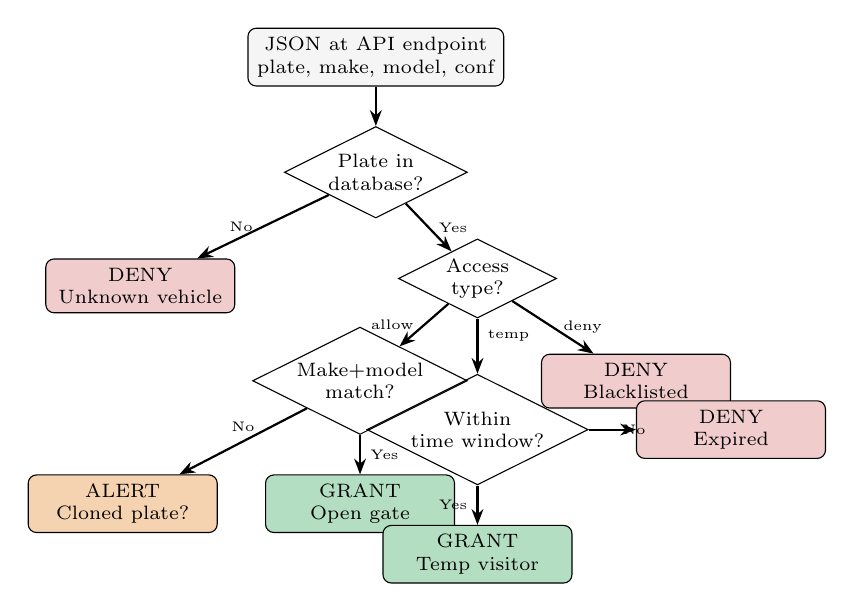
\begin{tikzpicture}[
    node distance=0.5cm and 0.8cm,
    box/.style={draw, rounded corners=3pt, align=center, font=\scriptsize,
                minimum width=2.4cm, minimum height=0.65cm},
    decision/.style={diamond, draw, aspect=2, align=center, font=\scriptsize,
                     inner sep=1pt},
    arr/.style={-{Stealth[length=2mm]}, thick},
    grantbox/.style={fill=grantgreen!35},
    denybox/.style={fill=denyred!25},
    alertbox/.style={fill=alertorange!35}
  ]
    \node[box, fill=boxinput] (json) {JSON at API endpoint\\plate, make, model, conf};
    \node[decision, below=of json] (q1) {Plate in\\database?};
    \node[box, denybox, below left=0.8cm and 1.2cm of q1] (unk) {DENY\\Unknown vehicle};
    \node[decision, below right=0.8cm and 0.2cm of q1] (q2) {Access\\type?};
    \node[decision, below left=0.7cm and 0.3cm of q2] (q3) {Make+model\\match?};
    \node[decision, below=0.7cm of q2] (q4) {Within\\time window?};
    \node[box, denybox, below right=0.7cm and 0.3cm of q2] (blk) {DENY\\Blacklisted};
    \node[box, grantbox, below=of q3] (gnode) {GRANT\\Open gate};
    \node[box, alertbox, left=0.6cm of gnode] (anode) {ALERT\\Cloned plate?};
    \node[box, grantbox, below=of q4] (temp) {GRANT\\Temp visitor};
    \node[box, denybox, right=0.6cm of q4] (exp) {DENY\\Expired};

    \draw[arr] (json) -- (q1);
    \draw[arr] (q1) -- node[left, font=\tiny]{No} (unk);
    \draw[arr] (q1) -- node[right, font=\tiny]{Yes} (q2);
    \draw[arr] (q2) -- node[left, font=\tiny]{allow} (q3);
    \draw[arr] (q2) -- node[right, font=\tiny]{deny} (blk);
    \draw[arr] (q2) -- node[right, font=\tiny,pos=0.3]{temp} (q4);
    \draw[arr] (q3) -- node[right, font=\tiny]{Yes} (gnode);
    \draw[arr] (q3) -- node[above, font=\tiny]{No} (anode);
    \draw[arr] (q4) -- node[left, font=\tiny]{Yes} (temp);
    \draw[arr] (q4) -- node[right, font=\tiny]{No} (exp);
  \end{tikzpicture}%
  }
\end{frame}

\begin{frame}[fragile]{Vehicle Database \& Access Types}
  \begin{columns}[T]
    \column{0.48\textwidth}
    \textbf{Storage:} \texttt{vehicles.json} (permanent rules)
    \begin{lstlisting}
{
  "licensePlate": "ABC-1234",
  "make": "Toyota",
  "model": "Corolla",
  "accessType": "allow",
  "ownerName": "John Doe"
}
    \end{lstlisting}
    \column{0.48\textwidth}
    \begin{block}{Access Types}
      \begin{tabular}{@{}p{1.2cm}p{4.5cm}@{}}
        \toprule
        \textbf{Type} & \textbf{Behavior} \\
        \midrule
        \texttt{allow} & Permanent whitelist $\rightarrow$ GRANT (after dual check) \\
        \texttt{deny}  & Permanent blacklist $\rightarrow$ DENY immediately \\
        \texttt{temp}  & Allowed only between \texttt{entryTime} and \texttt{expiry} \\
        \bottomrule
      \end{tabular}
    \end{block}
    \textbf{Roles:}
    \begin{itemize}
      \item \textbf{Admin:} add allow / deny / temp rules
      \item \textbf{User:} add temp visitors only
      \item Manual override via dashboard
    \end{itemize}
  \end{columns}
\end{frame}

%==============================================================================
\section{Results}
%==============================================================================

\begin{frame}{Quantitative Results}
  \centering
  \begin{tabular}{@{}lcccc@{}}
    \toprule
    \textbf{Model} & \textbf{Precision} & \textbf{Recall} & \textbf{mAP@0.5} & \textbf{Notes} \\
    \midrule
    YOLOv8n LPD & 98.50\% & 95.53\% & 98.07\% & Epoch 50, imgsz 384 \\
    YOLOv8n Char & 98.99\% & 96.88\% & 98.07\% & Epoch 100, imgsz 640 \\
    EfficientNet-B4 VMMR & --- & --- & --- & Top-1: 96.24\%, Top-5: 99.39\% \\
    \bottomrule
  \end{tabular}
  \vspace{0.8em}

  \begin{columns}[T]
    \column{0.32\textwidth}
    \begin{block}{LPD Strength}
      High precision (98.5\%) --- few false plate detections at gate.
    \end{block}
    \column{0.32\textwidth}
    \begin{block}{OCR Strength}
      38-class char detector handles Pakistani plate formats.
    \end{block}
    \column{0.32\textwidth}
    \begin{block}{VMMR Strength}
      245-class fine-grained recognition with 96\%+ Top-1 on 17K test images.
    \end{block}
  \end{columns}
\end{frame}

\begin{frame}{Qualitative Results}
  \textbf{Demonstrated capabilities:}
  \begin{itemize}
    \item Fog/haze images: visible improvement after DCP defog before LPD
    \item Rain scenes: vertical streak suppression preserves plate characters
    \item Night frames: CLAHE + gamma restores plate readability
    \item Multi-plate parking scenes: LPD detects multiple boxes
    \item Annotated output: vehicle label (yellow) + plate box (lime) + text
  \end{itemize}
  \vspace{0.4em}
  \begin{alertblock}{Integrated pipeline}
    Single notebook chains preprocessing $\rightarrow$ VMMR $\rightarrow$ LPD $\rightarrow$ OCR
    $\rightarrow$ formatted plate string with side-by-side before/after grids.
  \end{alertblock}
\end{frame}

%==============================================================================
\section{Conclusion}
%==============================================================================

\begin{frame}{Limitations \& Future Work}
  \begin{columns}[T]
    \column{0.48\textwidth}
    \textbf{Current limitations:}
    \begin{itemize}
      \item $\sim$1 image/sec on Pi --- not 30\,FPS continuous web stream
      \item Wi-Fi needed for Vercel upload (AI runs offline on Pi)
      \item Optional GPIO/LED only --- not certified industrial gate motor
      \item Accuracy drops in extreme weather or poor camera setup
      \item Event storage on Vercel may reset on cold start/redeploy
    \end{itemize}
    \column{0.48\textwidth}
    \textbf{Already implemented (not limitations):}
    \begin{itemize}
      \item Orange Pi edge deployment + 3 models
      \item End-to-end latency $\leq$2\,s ($\sim$700--1000\,ms)
      \item Pi $\rightarrow$ Vercel via \texttt{gate\_sync.py}
      \item Database allow/deny/temp $\rightarrow$ gate opened/closed
      \item Live Feed dashboard on Vercel
    \end{itemize}
  \end{columns}
\end{frame}

\begin{frame}{Conclusion}
  \begin{block}{Summary}
    We built an end-to-end \textbf{all-weather smart vehicle gate} system that combines:
    \begin{enumerate}
      \item Classical weather restoration (fog, rain, night)
      \item Two-stage YOLOv8n license plate reading
      \item EfficientNet-B4 vehicle make--model recognition (245 classes)
      \item Dual-modality access control (plate + vehicle identity)
      \item Edge deployment on Orange Pi with web dashboard
    \end{enumerate}
  \end{block}
  \vspace{0.5em}
  \centering
  \Large\textbf{Thank You}\\[0.4em]
  \normalsize Questions?
\end{frame}

\end{document}
